\section{Homework 8}

\subsection{信号调制与解调}

\subsubsection{绘制波形与频谱}

(1)$\cos(\Omega_1 t)$的频谱为$\pi[\delta(\omega+\Omega_1)+\delta(\omega-\Omega_1
)]$, 因此$Y_1(\omega)=\frac{1}{2}[F(\omega+\omega_c)+F(\omega-\omega_c)]=
\frac{\pi}{2}[\delta(\omega-5\Omega_1)+\delta(\omega-3\Omega_1)+\delta(\omega+3
\Omega_1)+\delta(\omega+5\Omega_1)]$.

比较$y_1,y_2$表达式, 由Fourier变换的线性性, 有$Y_2(\omega)=0.8Y_1(\omega)+\pi
[\delta(\omega-\omega_c)+\delta(\omega+\omega_c)]=
\pi[0.4\delta(\omega-5\Omega_1)+\delta(\omega-4\Omega_1)+0.4\delta(\omega-3\Omega_1)
+0.4\delta(\omega+3\Omega_1)+\delta(\omega+4\Omega_1)+0.4\delta(\omega+5\Omega_1)]$

其时域和频域信号波形如图\ref{fig:8-1-1-1}所示

\begin{figure*}[htbp]
    \centering
    \includegraphics[width=0.7\textwidth]{images/8-1-1-1.png}
    \caption{8-1-1(1)波形}\label{fig:8-1-1-1}
\end{figure*}

(2)波形如图\ref{fig:8-1-1-2}所示. 图中可见包络线检波丢失了检波前信号的一个小峰值.

\begin{figure*}[htbp]
    \centering
    \includegraphics[width=0.7\textwidth]{images/8-1-1-2.png}
    \caption{8-1-1(2)波形}\label{fig:8-1-1-2}
\end{figure*}

\subsubsection{单边带解调}

如图\ref{fig:8-1-2}.

\begin{figure*}[htbp]
    \centering
    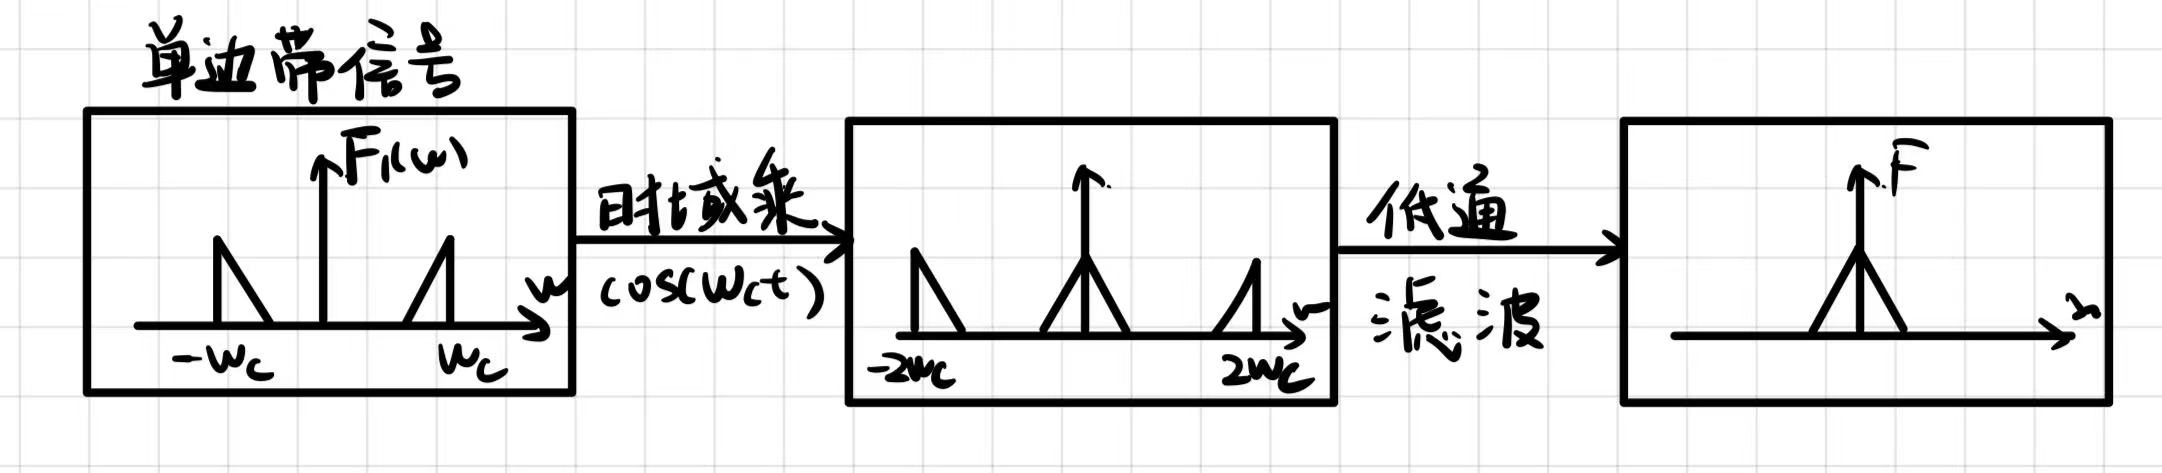
\includegraphics[width=0.8\textwidth]{images/8-1-2.jpg}
    \caption{8-1-2示意图}\label{fig:8-1-2}
\end{figure*}

\subsection{信号调制系统分析}

\subsubsection{第一小题}

(1) $h(t)=\mathcal{F}^{-1}[\mathcal{F}[\cos(\omega_ct)\delta(t)]H_L(\omega)]=
\displaystyle\frac{3\Omega}{2\pi}\operatorname{Sa}(\frac{3\Omega t}{2})$

(2) $Sa(\Omega t)$的频谱为$\frac{\pi}{\Omega}[u(t+\Omega)-u(t-\Omega)]$,
$\cos(\omega_c t + \frac{\pi}{2})\cos(\omega_ct)$的频谱为
$-\frac{j\pi}{2}[\delta(\omega-2\omega_c)+\delta(\omega+2\omega_c)]$, 因此二者卷积
后滤波的结果为$0$.

(3) 相当于$2$的结果加负号, 结果仍然为$0$.

(4) 线性, 因为相乘和滤波操作都为线性; 时变, 因为如果令输入信号等于
$\delta(t-\frac{\pi}{2\omega_c})$, 则其结果为
$\mathcal{F}^{-1}[\mathcal{F}[\cos(\omega_ct)
\delta(t-\frac{\pi}{2\omega_c})]H_L(\omega)]=\displaystyle\mathcal{F}^{-1}[0\cdot 
H_L(\omega)]=0\ne h(t-\pi/2\omega_c)$.

\subsection{第二小题}

进入带通滤波器的频谱为$\frac{1}{2\pi}[X(\omega)*X(\omega)+\pi X(\omega-\omega_c)
+\pi X(\omega+\omega_c)+\pi^2\delta(\omega-2\omega_c)+2\pi^2\delta(\omega)+
\pi^2\delta(\omega+2\omega_c)]$. 我们希望保留频谱中的$\frac{1}{2}[X(\omega+\omega_c)
+X(\omega-\omega_c)]$项, 因此取$A=1,\omega_l=\omega_c-\omega_M,\omega_h=\omega_c+
\omega_M$. 此时要求剩余项的频谱不能侵入带通滤波器可以滤过的区域, 有关系式$
\omega_l=\omega_c-\omega_M>2\omega_M,\omega_h=\omega_c+\omega_M<2\omega_c$, 即
$\omega_c>3\omega_M$

\subsection{信号采样}

\subsubsection{信号脉冲编码调制}

$f(t)$在$[12,116]$之间取值, 大约在$343\cdot35\mathrm{mV}$到$3314\cdot35\mathrm{mV}$
之间, 共有$2971$个量化等级, 因此$N>\log_22971\approx11.53$, 因此最少要$12$位编码.

\subsection{证明题}

只需要证明二者在频域下能量相等, 即$\displaystyle\int_{-\infty}^{+\infty}
||F(\omega)||^2\,\mathrm{d}\omega=\int_{-\infty}^{+\infty}||\bar{F}(\omega)||^2
\,\mathrm{d}\omega$. 由于$\bar{F(\omega)}=F(\omega)\cdot j\operatorname{sgn}(
-\omega)$, 因此在$\omega\ne0$时$|F(\omega)|=|\bar{F}(\omega)|$, 二者不相等的点构成
一个零测度集, 不影响积分结果, 因此$\displaystyle\int_{-\infty}^{+\infty}
||F(\omega)||^2\,\mathrm{d}\omega=\int_{-\infty}^{+\infty}||\bar{F}(\omega)||^2
\,\mathrm{d}\omega$, 推出二者在时域下的能量也相等: $\displaystyle
\int_{-\infty}^{+\infty}|f(t)|^2\,\mathrm{d}t=\int_{-\infty}^{+\infty}
|\bar{f}(t)|^2\,\mathrm{d}t$


        